% Created 2019-08-27 Tue 19:52
% Intended LaTeX compiler: pdflatex
\documentclass[presentation]{beamer}
\usepackage[utf8]{inputenc}
\usepackage[T1]{fontenc}
\usepackage{graphicx}
\usepackage{grffile}
\usepackage{longtable}
\usepackage{wrapfig}
\usepackage{rotating}
\usepackage[normalem]{ulem}
\usepackage{amsmath}
\usepackage{textcomp}
\usepackage{amssymb}
\usepackage{capt-of}
\usepackage{hyperref}
\usepackage{color}
\usepackage{listings}
\usecolortheme{Imperial}
\usepackage{booktabs}
\usepackage{caption}
\usepackage{subcaption}
\usepackage{amsfonts}
\usepackage{epstopdf}
\usepackage{multimedia}
\usepackage{datetime}
\let\dateUKenglish\relax
\newdateformat{dateUKenglish}{\THEDAY~\monthname[\THEMONTH] \THEYEAR}
\institute{
\includegraphics[height=0.7cm]{Imperial_1_Pantone_solid.eps}}
\setbeamerfont{caption}{size=\scriptsize}
\usetheme{default}
\author{Paul Bartholomew, Sylvain Laizet}
\date{\today}
\title{Scale-Resolving Simulations of Three-Dimensional Gravity Currents Beyond the Boussinesq Limit}
\hypersetup{
 pdfauthor={Paul Bartholomew, Sylvain Laizet},
 pdftitle={Scale-Resolving Simulations of Three-Dimensional Gravity Currents Beyond the Boussinesq Limit},
 pdfkeywords={},
 pdfsubject={},
 pdfcreator={Emacs 25.2.2 (Org mode 9.2.3)}, 
 pdflang={English}}
\begin{document}

\maketitle
\begin{frame}{Outline}
\tableofcontents
\end{frame}


\section{Introduction}
\label{sec:org05f97a0}

\begin{frame}[label={sec:org948e9d8}]{Gravity Currents}
\begin{center}
\includegraphics[width=\columnwidth]{./figures/intro-grav-curr.png}
\end{center}
\end{frame}

\begin{frame}[label={sec:orgca8aebf}]{Gravity Currents is 2D valid?}
\begin{itemize}
\item Gravity currents commonly associated with destructive events
\item Previous work by \cite{Espath2014} showed different behaviour for 2D and 3D simulations in
Boussinesq limit
\end{itemize}

\begin{equation*}
  \frac{D\boldsymbol{u}}{Dt} = -\boldsymbol{\nabla}p + \boldsymbol{\nabla}\cdot\boldsymbol{\tau} +
  \Delta{}\rho \boldsymbol{g}
\end{equation*}

\begin{itemize}
\item Literature claims 2D simulations sufficient for non-Boussinesq
\begin{itemize}
\item \alert{N.B.} requires long time simulation
\end{itemize}
\end{itemize}
\end{frame}

\section{Numerical Methods}
\label{sec:org1743ad3}

\begin{frame}[label={sec:org0705b60},fragile]{Xcompact3d}
 \begin{columns}
\begin{column}{0.5\columnwidth}
\begin{itemize}
\item New codebase, uniting multiple projects in \texttt{Incompact3d}
\item High-order compact finite difference code
\item Highly scalable, strong scaling up to \(\mathcal{O}\left(10^{5}\right)\) CPUs using \texttt{decomp2d}
\end{itemize}
\end{column}

\begin{column}{0.5\columnwidth}
\begin{center}
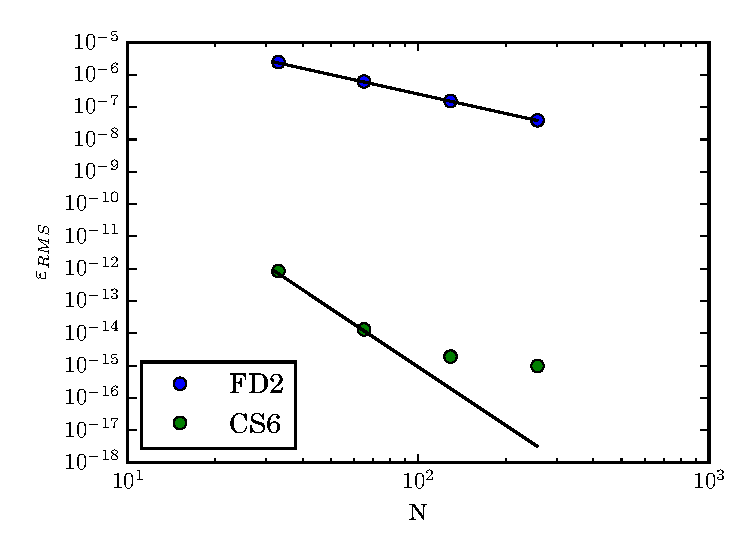
\includegraphics[width=0.8\columnwidth]{./figures/convergence-tgv2d.eps}
\end{center}

\begin{center}
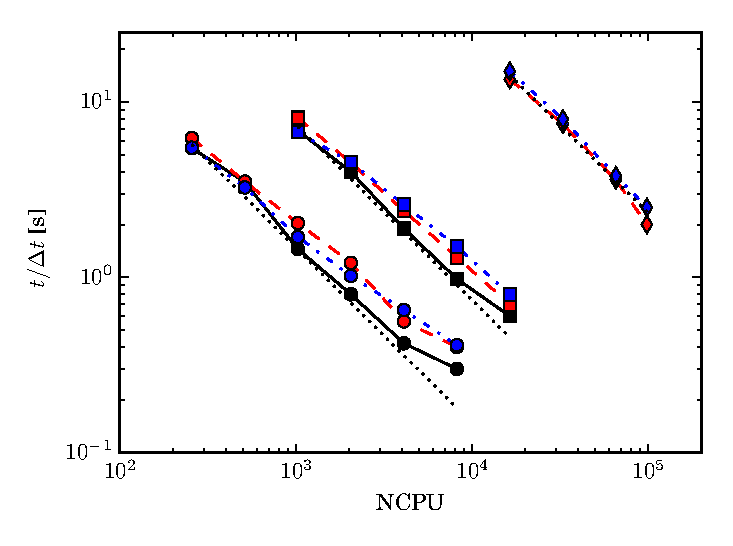
\includegraphics[width=0.8\columnwidth]{./figures/x3d-scaling.eps}
\end{center}
\end{column}
\end{columns}
\end{frame}

\begin{frame}[label={sec:org772d5ba}]{Xcompact3d LMN}
\begin{columns}
\begin{column}{0.5\columnwidth}
Extended with variable-density solver to solve LMN approximation \cite{Bartholomew2019}
\begin{align*}
  \rho \frac{D\boldsymbol{u}}{Dt} &= -\boldsymbol{\nabla} p +
                                    \boldsymbol{\nabla}\cdot\boldsymbol{\tau} + \rho\boldsymbol{g}
  \\
  \frac{D\rho}{Dt} &= -\rho\boldsymbol{\nabla}\cdot\boldsymbol{u} \\
  p^{\left(0\right)} &= \rho T,\ \boldsymbol{\nabla} p^{\left(0\right)} = 0
\end{align*}
\end{column}

\begin{column}{0.5\columnwidth}
\begin{figure}[htbp]
\centering
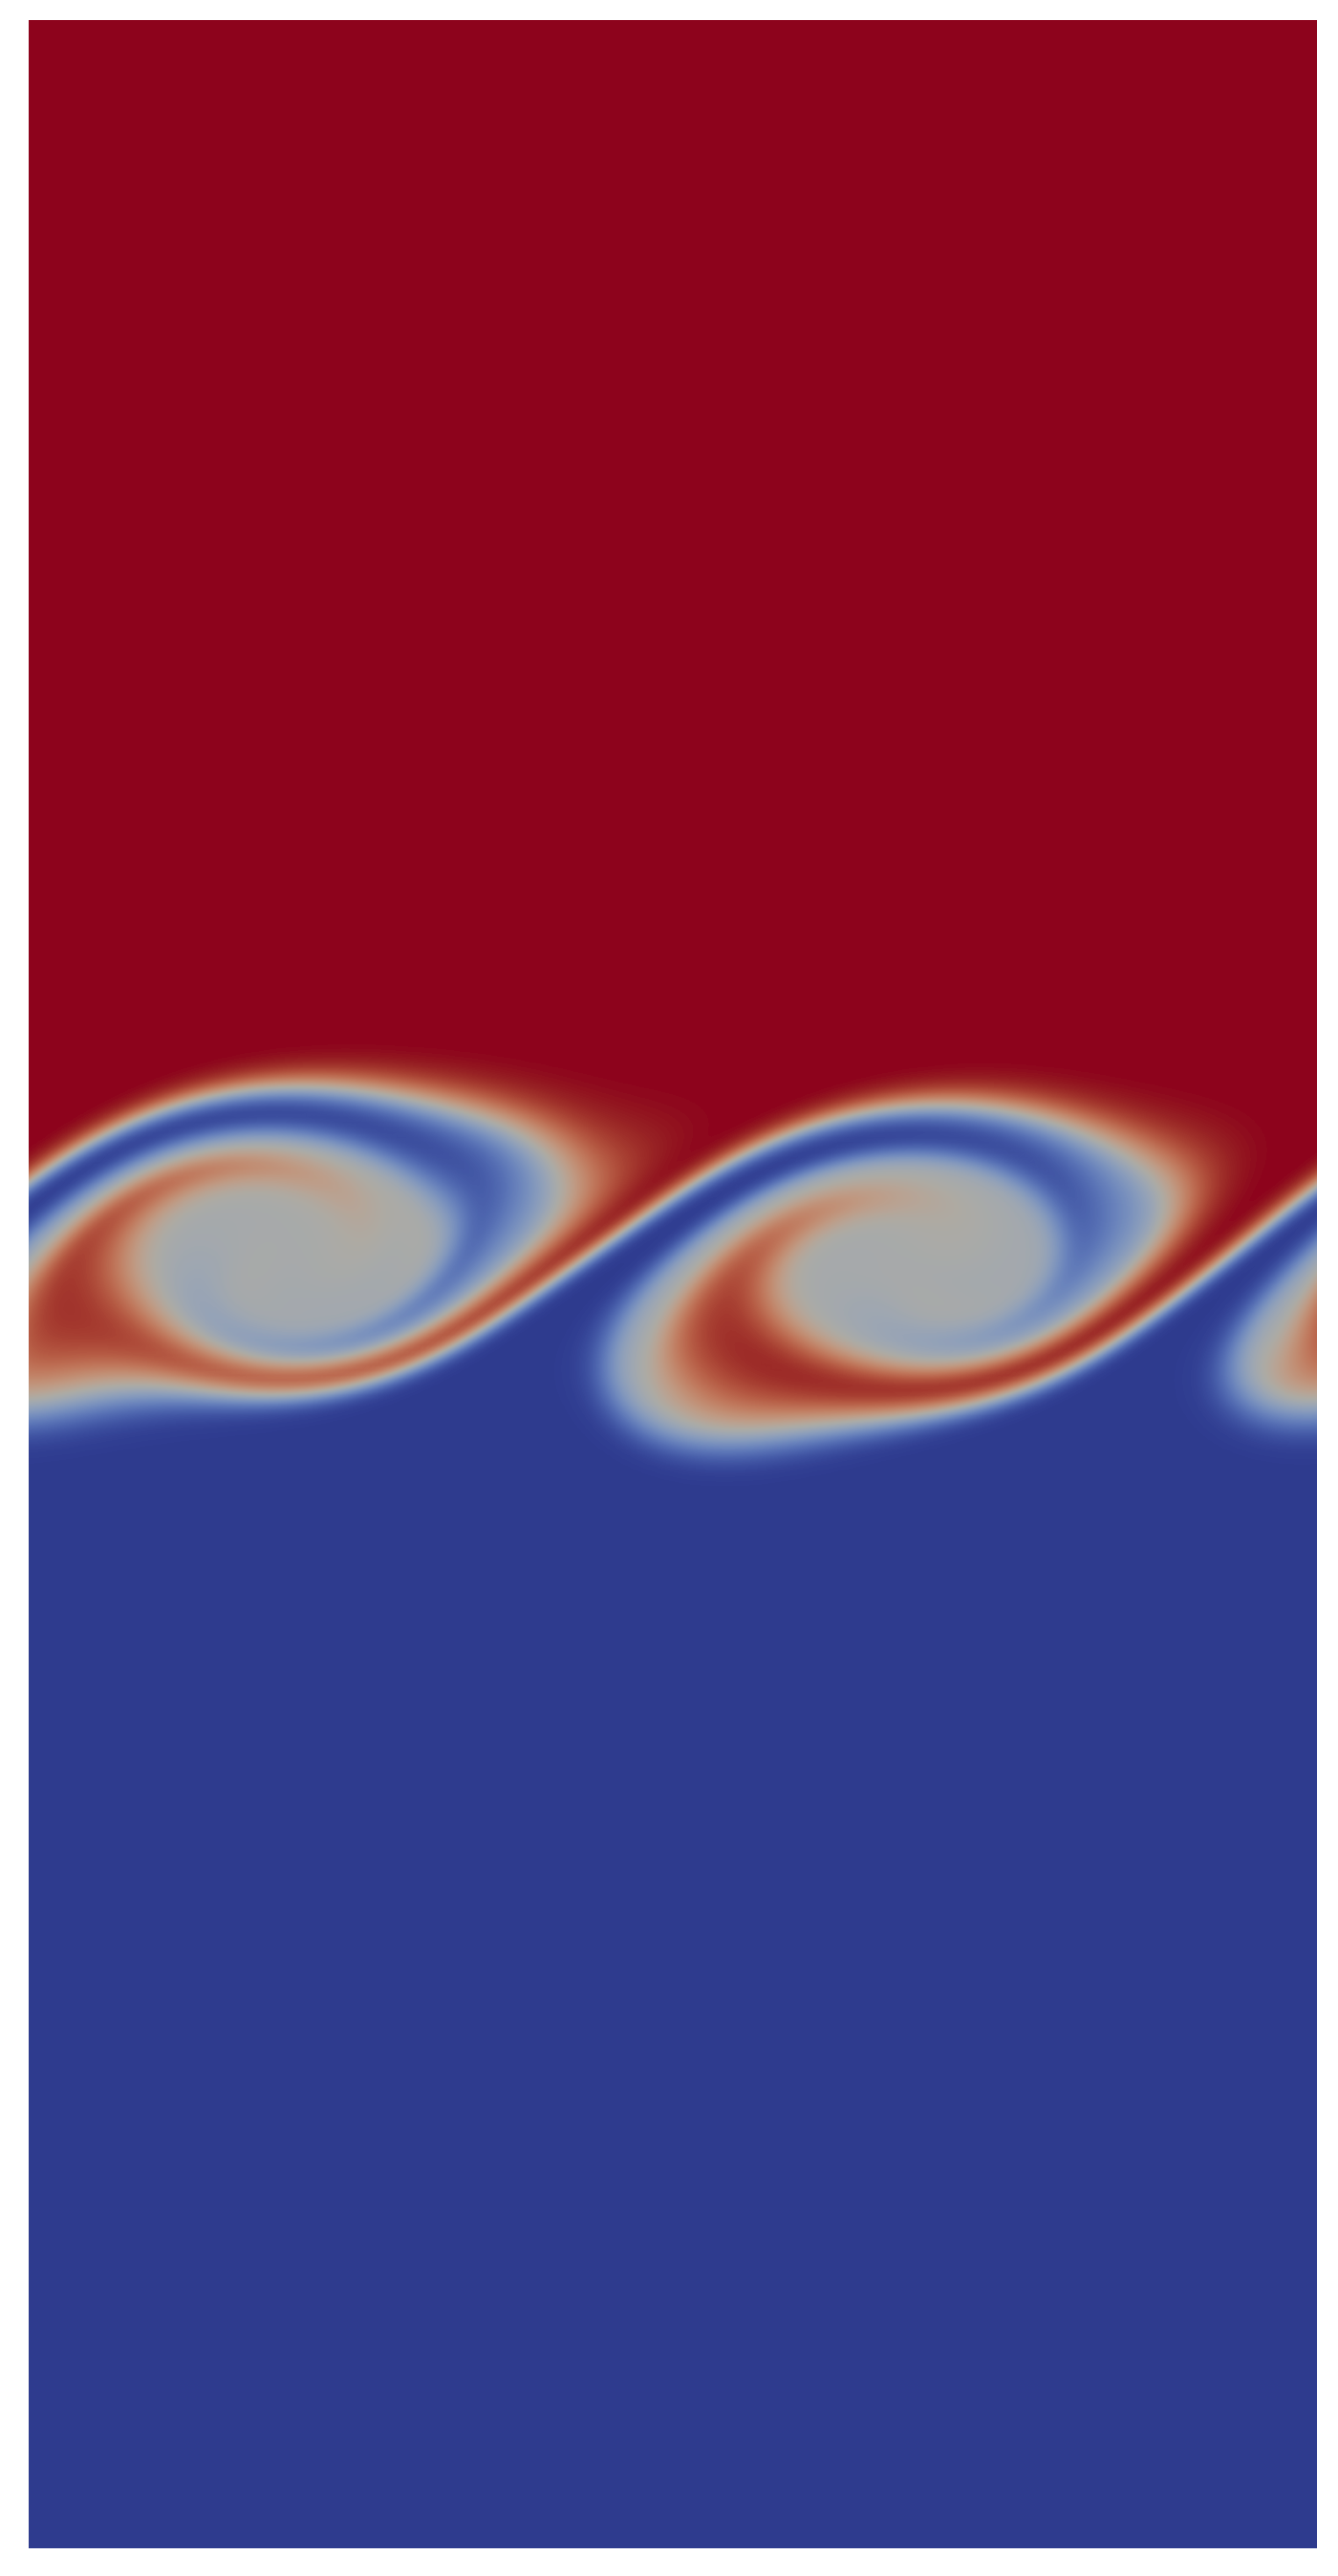
\includegraphics[width=0.7\columnwidth]{./figures/mixlayer.png}
\caption{Hot/cold mixing layer}
\end{figure}
\end{column}
\end{columns}
\end{frame}


\begin{frame}[label={sec:orgb3c64f4}]{Simulating gravity currents}
\begin{itemize}
\item Variable-density solver doesn't require ideal gas law
\item Can use arbitrary EOS
\item To verify, test against \cite{Birman2005} for Boussinesq and non-Boussinesq cases
\end{itemize}
\begin{align*}
  \rho \left( c \right) &= c \left( \rho_1 - \rho_2 \right) + \rho_2 \\
  \boldsymbol{\nabla}\cdot\boldsymbol{u} &= 0 \\
  \Rightarrow \frac{D\rho}{Dt} &= \frac{1}{ReSc} {\boldsymbol{\nabla}}^2 \rho
\end{align*}
\end{frame}
\section{Results}
\label{sec:org6bf3b24}

\begin{frame}[label={sec:org9cb657e}]{2D lock-exchange validation}
\begin{equation*}
  \begin{split}
    \boldsymbol{u} \left( \boldsymbol{x}, t=0 \right) &= \boldsymbol{0}\\
    \rho \left( x, t=0 \right) &=
    \begin{cases}
      \rho_1 & x \leq 14 \\
      \rho_2 & \mbox{otherwise}
    \end{cases}
  \end{split}
\end{equation*}

\begin{figure}[htbp]
\centering
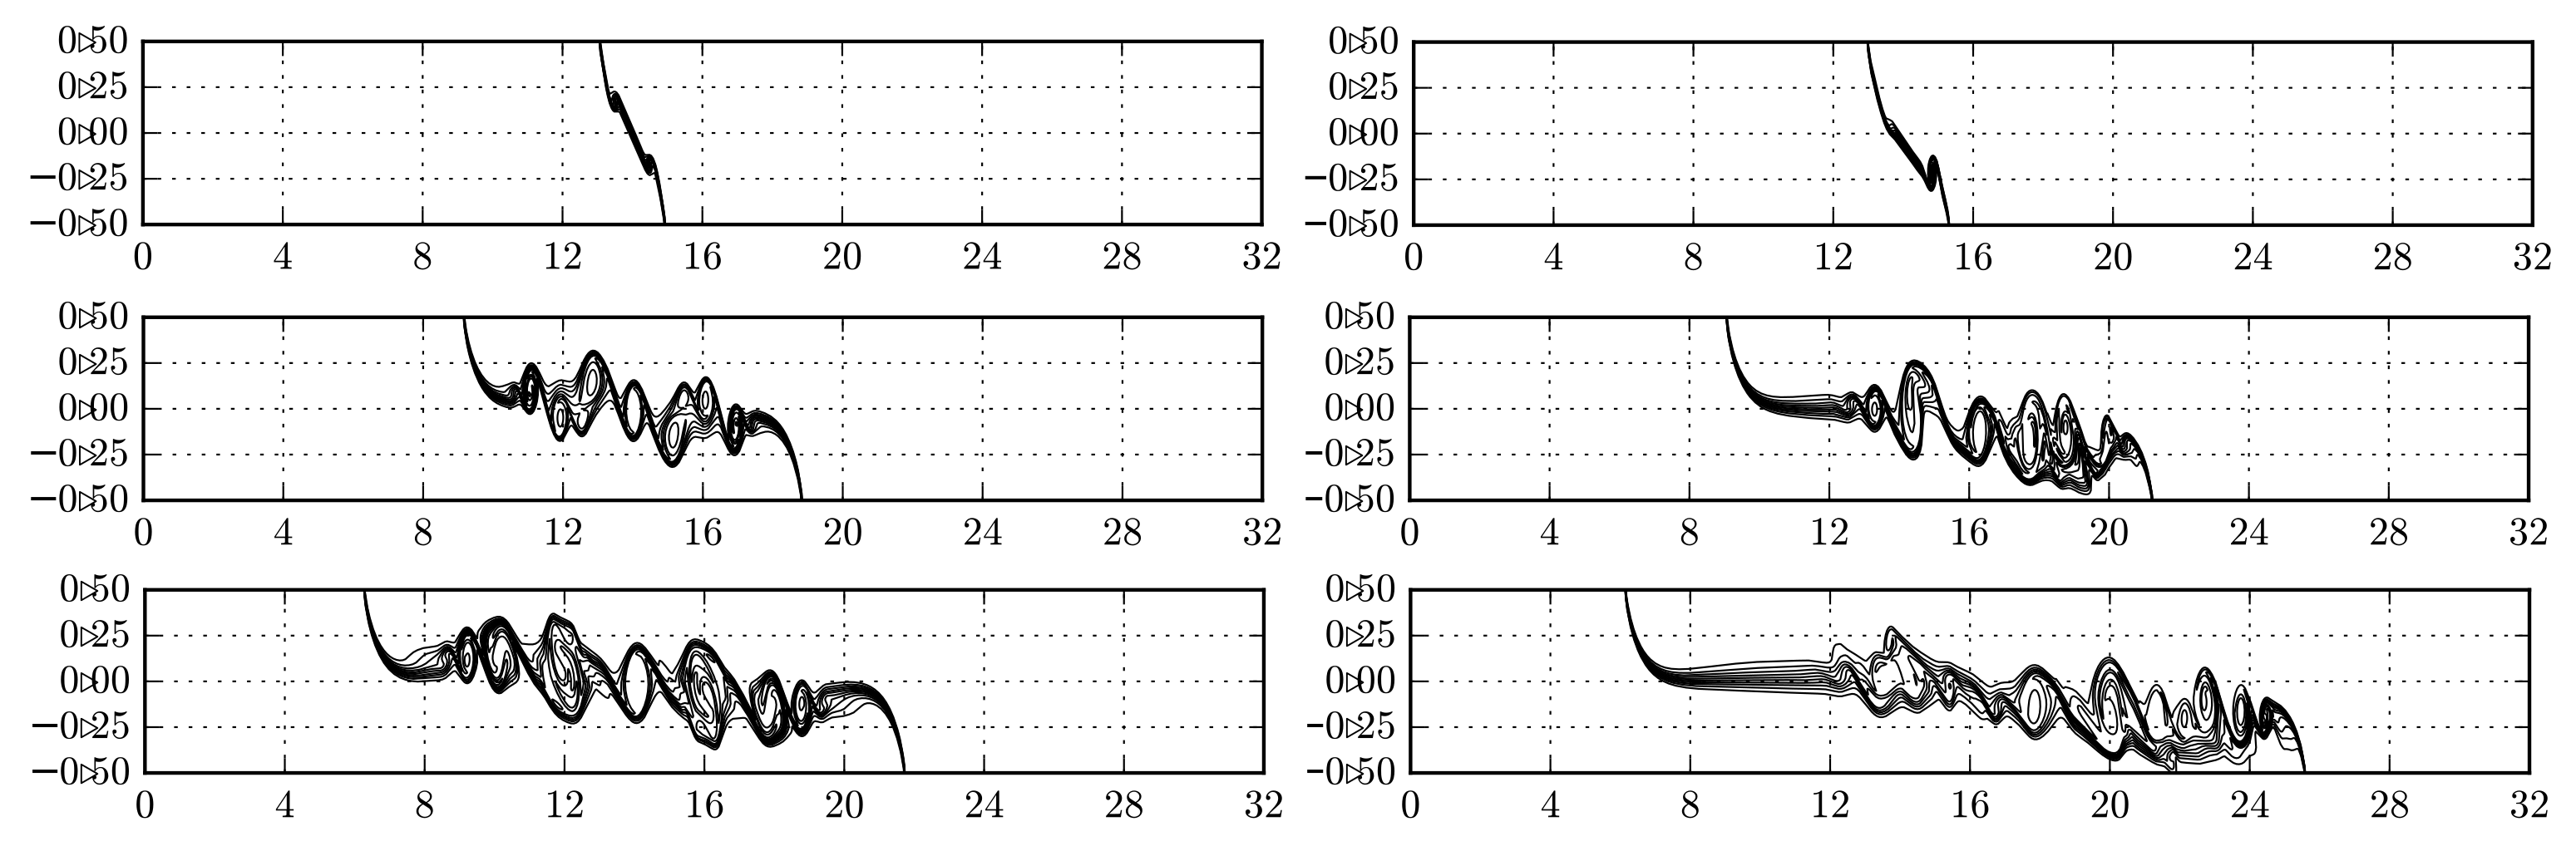
\includegraphics[width=.9\linewidth]{./figures/2d-lockexch.png}
\caption{Time evolution of Boussinesq and non-Boussinesq 2D lock-exchange}
\end{figure}
\end{frame}

\begin{frame}[label={sec:org0863305}]{2D lock-exchange validation}
\begin{figure}[htbp]
\centering
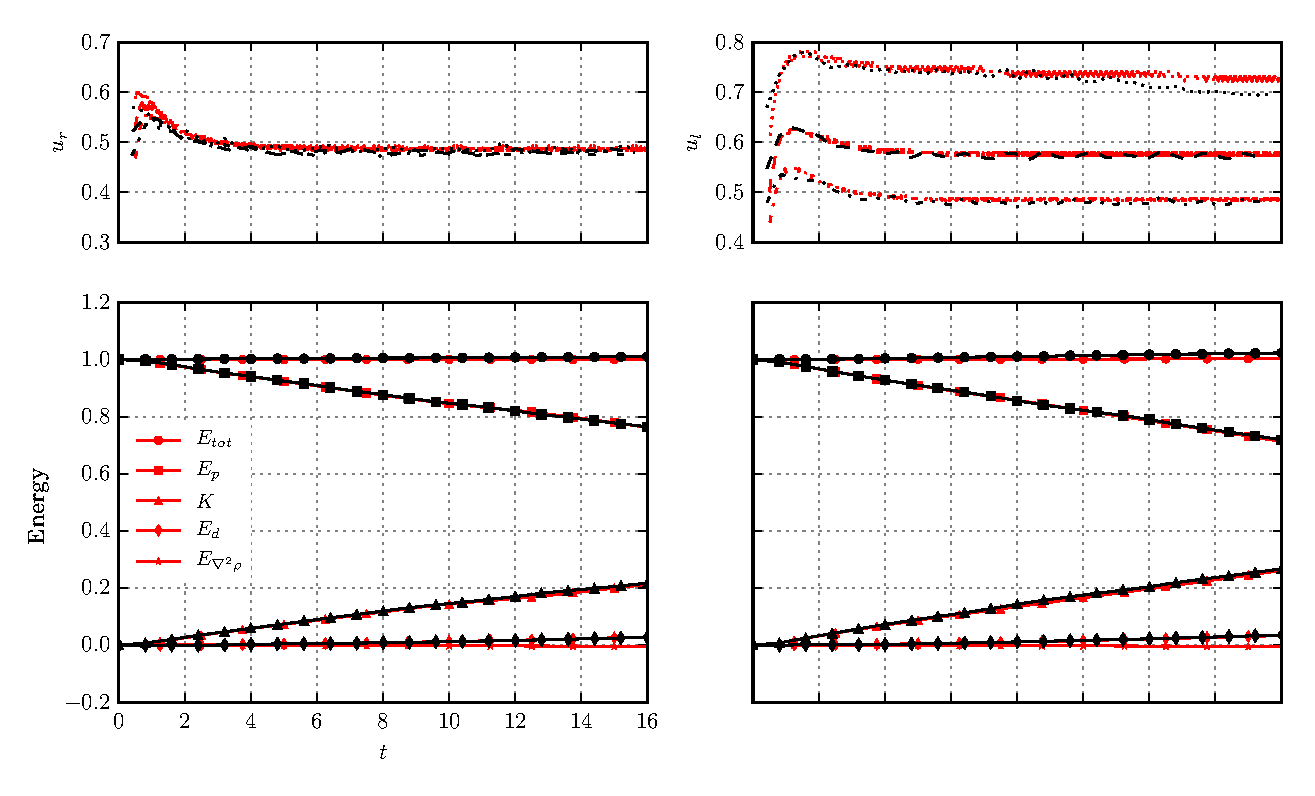
\includegraphics[width=.9\linewidth]{./figures/front_velocity_ebudg_veri.eps}
\caption{Comparison of front velocities and energy budgets for 2D lock-exchange}
\end{figure}
\end{frame}

\begin{frame}[label={sec:orgd3bab12}]{3D snapshots}
\begin{figure}[htbp]
\centering
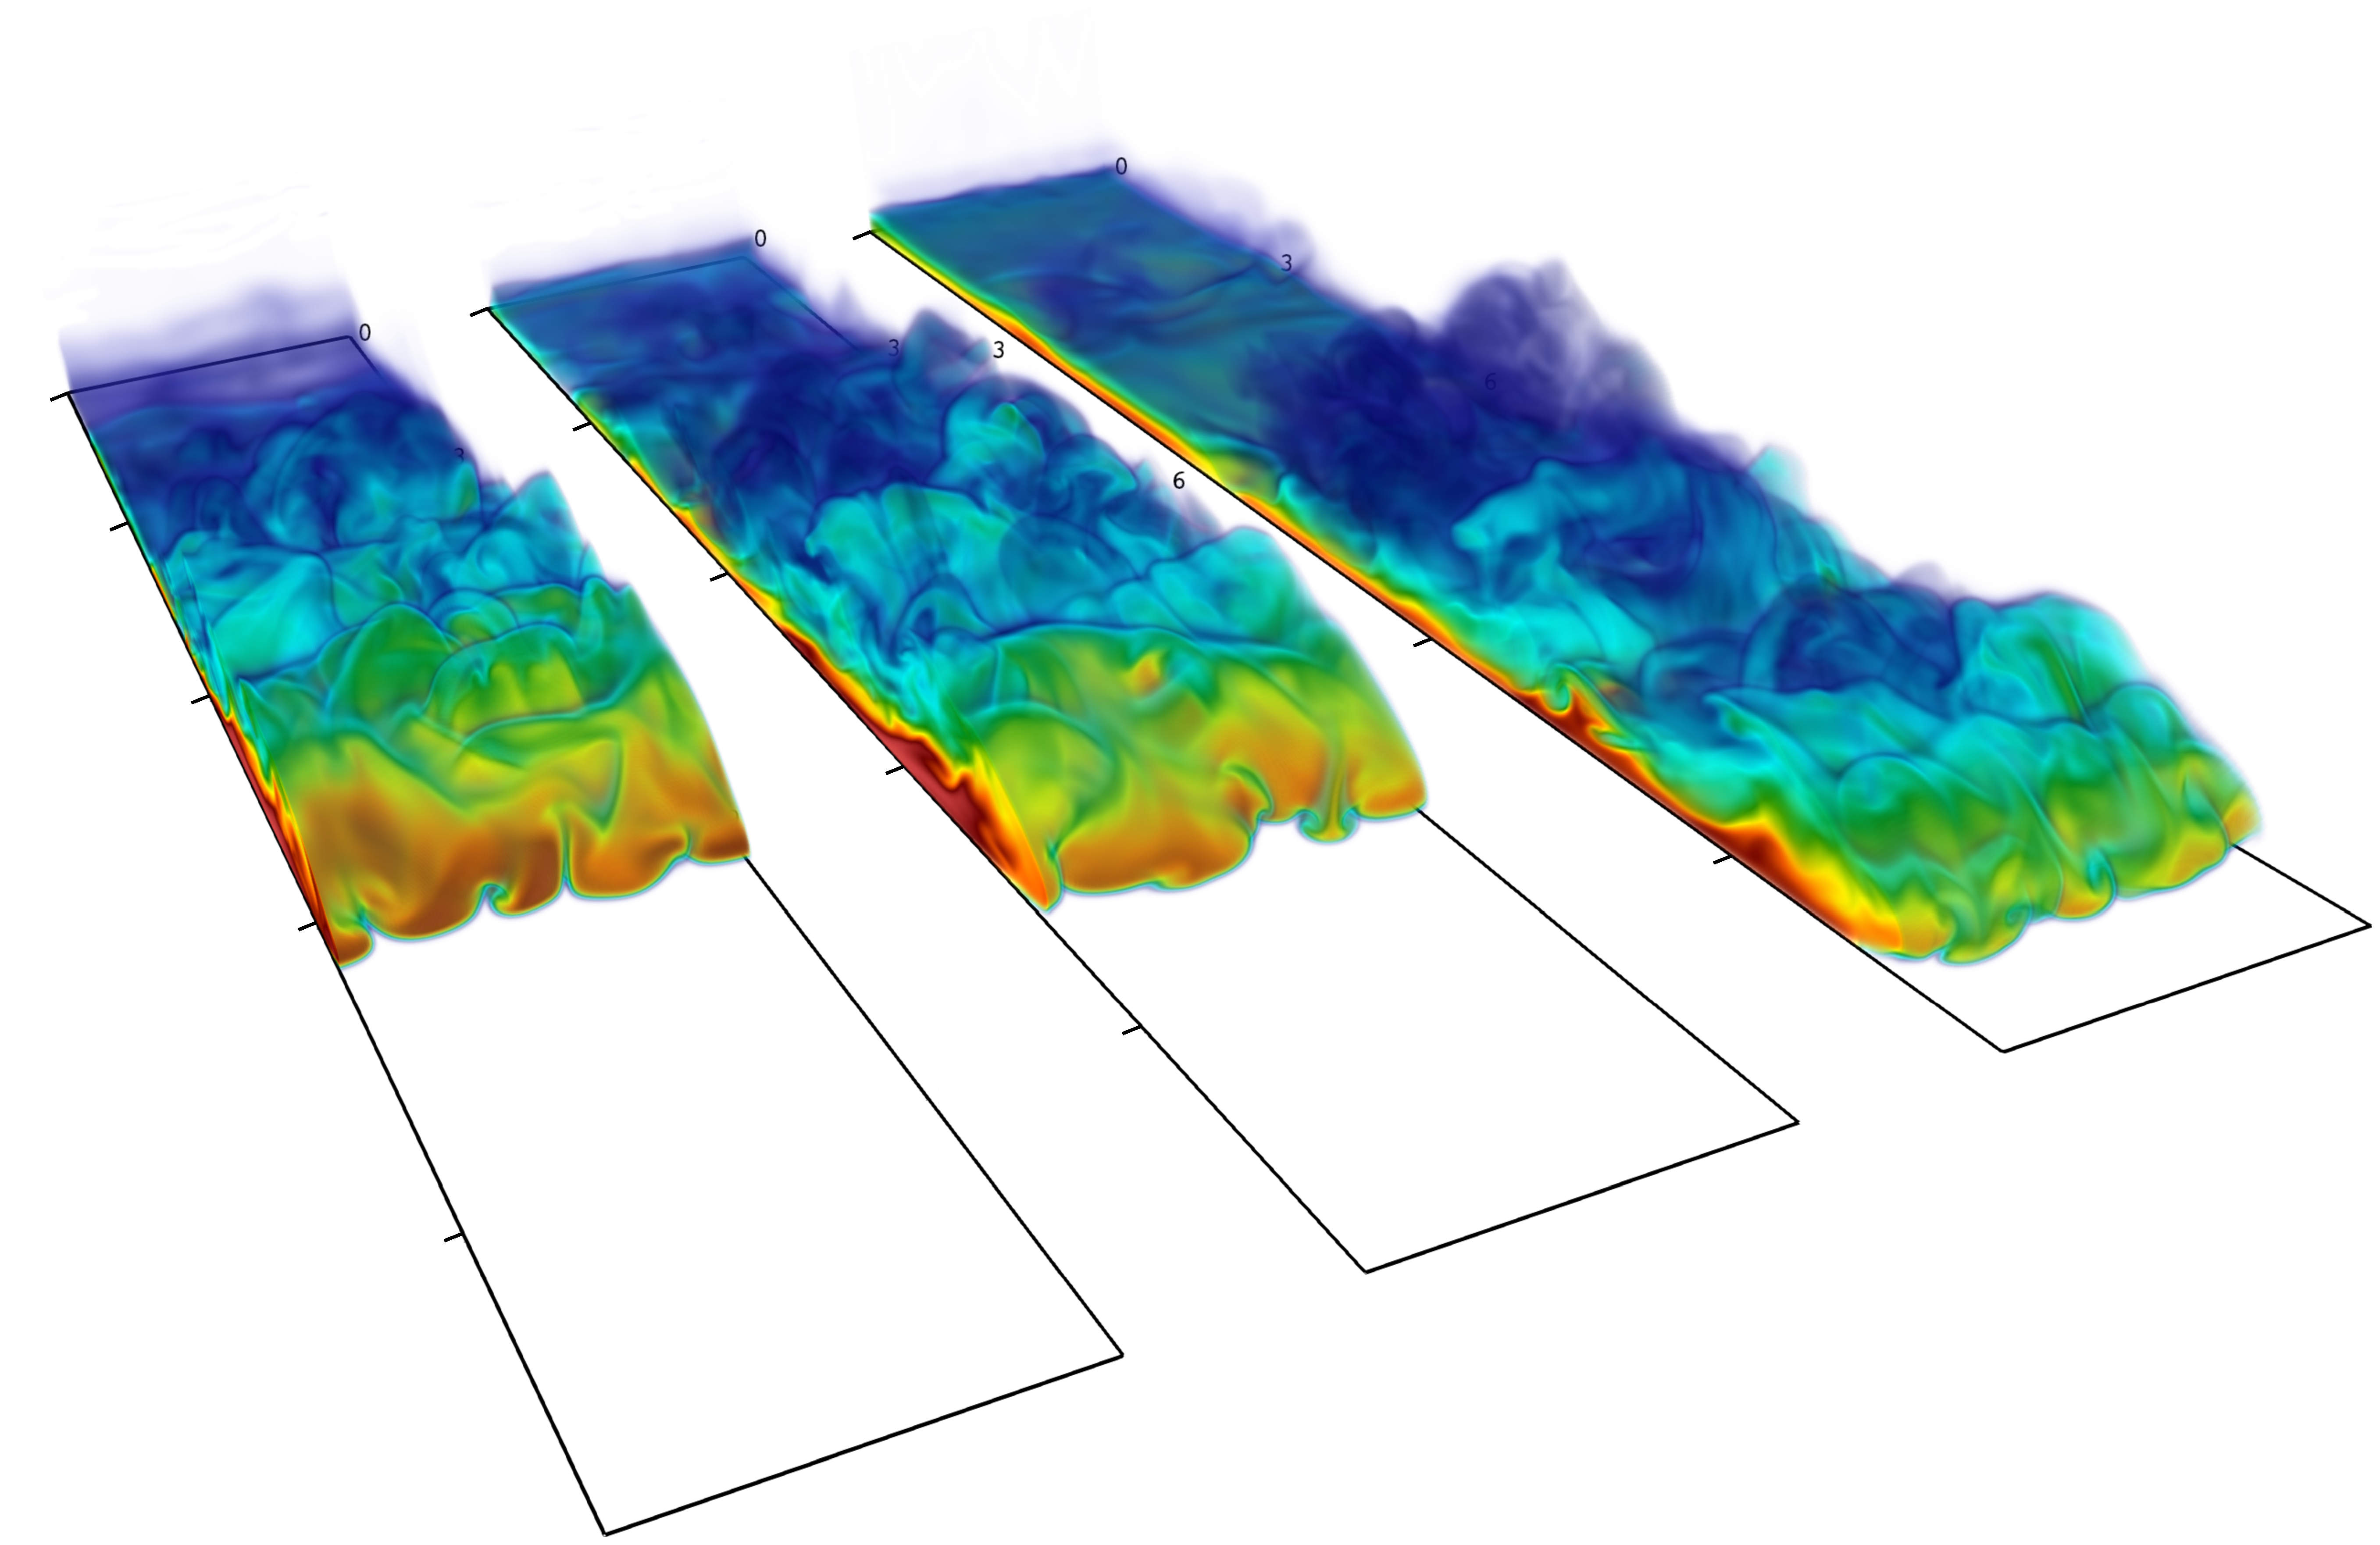
\includegraphics[width=0.9\textwidth]{./figures/3D_view.eps}
\caption{Concentration field at \(t=15\), \(\rho2/\rho1=0.998, 0.7, 0.4\)}
\end{figure}
\end{frame}

\begin{frame}[label={sec:orgddeb3a6}]{2D vs 3D comparison}
\begin{columns}
\begin{column}{0.5\columnwidth}
\begin{itemize}
\item Contours of \(c=0.9\) at \(t=15\)
\item 2D front consistently led by 3D depth-averaged front for all density ratios
\item Note structure in 2D contours
\end{itemize}
\end{column}

\begin{column}{0.5\columnwidth}
\begin{figure}[htbp]
\centering
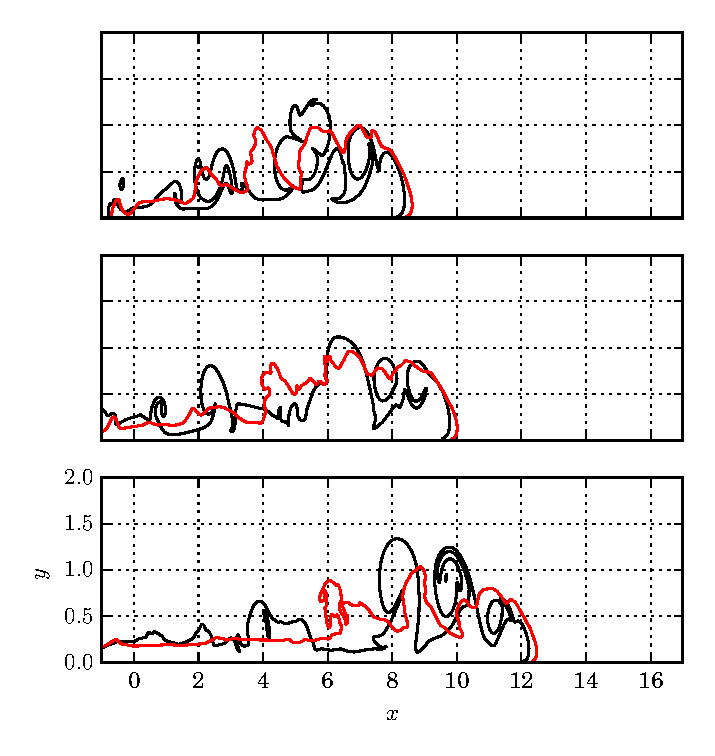
\includegraphics[width=0.9\columnwidth]{./figures/c09-2d3d-t15.eps}
\caption{2D (black) \& 3D (red) concentration contours}
\end{figure}
\end{column}
\end{columns}
\end{frame}

\begin{frame}[label={sec:orgc45dc6b}]{Evolution of front location}
\begin{figure}[htbp]
\centering
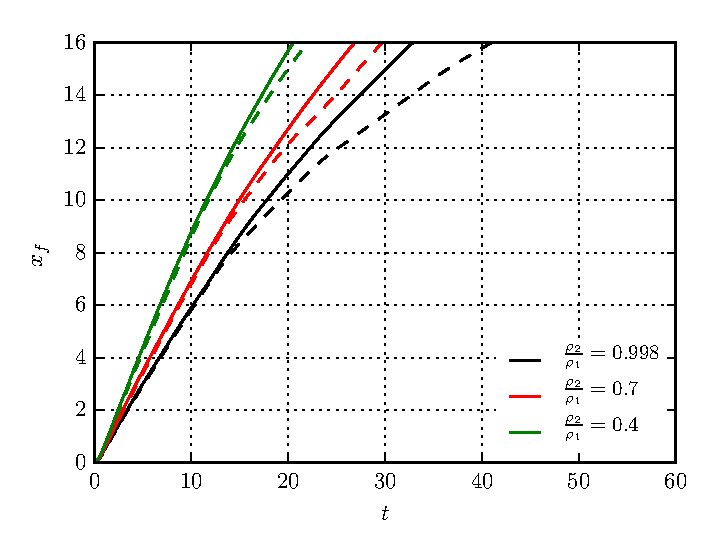
\includegraphics[width=0.7\textwidth]{./figures/2d3d_front_comparison.eps}
\caption{Evolution of 2D and 3D fronts}
\end{figure}
\end{frame}

\section{Conclusions}
\label{sec:org929b556}

\begin{frame}[label={sec:orgd0ca15b}]{Conclusion \& future work}
\begin{columns}
\begin{column}{0.5\columnwidth}
\begin{itemize}
\item Variable-density solver in \texttt{Xcompact3d} framework used to simulate non-Boussinesq gravity
currents
\item Comparison of 2D and 3D solutions shows different behaviour
\begin{itemize}
\item Speed of 3D current is increased
\item Apparent dependency on density ratio
\end{itemize}
\end{itemize}
\end{column}

\begin{column}{0.5\columnwidth}
\begin{itemize}
\item Investigate over longer times
\item Investigate for higher Reynolds numbers
\item Investigate using free surface solver
\end{itemize}
\end{column}
\end{columns}
\end{frame}

\section{Code availability}
\label{sec:org6f1cd98}

\begin{frame}[label={sec:orgda36814},fragile]{Code availability}
 \begin{itemize}
\item Xcompact3d is available at: \url{https://github.com/xcompact3d/Incompact3d}
\item Release preview on the \texttt{release} branch
\end{itemize}

\begin{figure}[htbp]
\centering
\includegraphics[width=\textwidth]{./figures/visu.png}
\caption{Examples using Xcompact3d}
\end{figure}
\end{frame}

\section{References}
\label{sec:org7ab960d}

\begin{frame}[label={sec:org2c9fd8c}]{References}
\bibliography{../../../../Documents/Postdoc}
\bibliographystyle{plain}
\end{frame}
\end{document}